\section{Chuyên Hạ Long, Quảng Ninh 25--26, Lần 1}

\caulc
\Opensolutionfile{ans}[ans/ans-26-2--SoGD-L1-LC]



\begin{ex}%[Dự án đề TT THPTQG2026]%[2D1H4-1]
	Đồ thị hàm số $y=\dfrac{2x-3}{x-1}$ có đường tiệm cận ngang là
	\choice
	{$x=-1$}
	{$y=-2$}
	{$x=1$}
	{\True $y=2$}
	\loigiai{
		Tập xác định $\mathscr{D} = \mathbb{R} \setminus \{1\}$.\\
		Ta có
		\[ \lim\limits_{x \to \pm\infty} y = \lim\limits_{x \to \pm\infty} \dfrac{2x-3}{x-1} = \lim\limits_{x \to \pm\infty} \dfrac{x\left(2-\dfrac{3}{x}\right)}{x\left(1-\dfrac{1}{x}\right)} = \lim\limits_{x \to \pm\infty} \dfrac{2-\dfrac{3}{x}}{1-\dfrac{1}{x}} = 2. \]
		Vì $\lim\limits_{x \to \pm\infty} y = 2$ nên đường thẳng $y=2$ là tiệm cận ngang của đồ thị hàm số.
	}
\end{ex}

%%%=============EX_2=============%%%
\begin{ex}%[Dự án đề TT THPTQG2026]%[1D2H3-3]
	Cho cấp số nhân $(u_n)$ có số hạng đầu $u_1=2$ và công bội $q=-3$. Tính $u_3$.
	\choice
	{\True $u_3=18$}
	{$u_3=54$}
	{$u_3=-18$}
	{$u_3=-54$}
	\loigiai{
		Ta có $u_3 = u_1 \cdot q^2 = 2 \cdot (-3)^2 = 18$.
	}
\end{ex}

%%%=============EX_3=============%%%
\begin{ex}%[Dự án đề TT THPTQG2026]%[2D3H2-2]
	Khảo sát thời gian tập thể dục của một số học sinh thu được mẫu số liệu ghép nhóm như sau:
	\begin{center}
		\begin{tabular}{|c|c|c|c|c|c|c|}
			\hline
			Thời gian (phút) & $[0;10)$ & $[10;20)$ & $[20;30)$ & $[30;40)$ & $[40;50)$ & $[50;60)$ \\ \hline
			Số học sinh & $10$ & $15$ & $22$ & $26$ & $20$ & $7$ \\ \hline
		\end{tabular}
	\end{center}
	Tính độ lệch chuẩn của mẫu số liệu ghép nhóm trên (\textit{làm tròn kết quả đến hàng đơn vị}).
	\choice
	{$12$}
	{\True $14$}
	{$15$}
	{$13$}
	\loigiai{
		Giá trị đại diện của các nhóm lần lượt là $c_1=5$, $c_2=15$, $c_3=25$, $c_4=35$, $c_5=45$, $c_6=55$.\\
		Tổng số học sinh là $n = 10+15+22+26+20+7 = 100$.\\
		Số trung bình là 
		\[\overline{x} = \dfrac{10\cdot5 + 15\cdot15 + 22\cdot25 + 26\cdot35 + 20\cdot45 + 7\cdot55}{100}= 30{,}2.\]
		Phương sai là
		\begin{eqnarray*}
			s^2 &=& \dfrac{1}{100} [10(5-30{,}2)^2 + 15(15-30{,}2)^2\\	
			&&+ 22(25-30{,}2)^2 + 26(35-30{,}2)^2+ 20(45-30{,}2)^2 + 7(55-30{,}2)^2]\\
			&=& 196{,}96
		\end{eqnarray*}
		Độ lệch chuẩn $s =\sqrt{s^2}= \sqrt{196{,}96} \approx 14$.		
	}
\end{ex}

%%%=============EX_4=============%%%
\begin{ex}%[Dự án đề TT THPTQG2026]%[1D1H5-3]
	Tập nghiệm của phương trình $\sin x = \dfrac{1}{2}$ là
	\choice
	{$\left\{ \dfrac{\pi}{3} + k2\pi; \dfrac{2\pi}{3} + k2\pi \mid k \in \mathbb{Z} \right\}$}
	{$\left\{ \dfrac{\pi}{6} + k\pi; \dfrac{5\pi}{6} + k\pi \mid k \in \mathbb{Z} \right\}$}
	{$\left\{ \dfrac{\pi}{3} + k\pi; \dfrac{2\pi}{3} + k\pi \mid k \in \mathbb{Z} \right\}$}
	{\True $\left\{ \dfrac{\pi}{6} + k2\pi; \dfrac{5\pi}{6} + k2\pi \mid k \in \mathbb{Z} \right\}$}
	\loigiai{
		Ta có 
		\[\sin x = \dfrac{1}{2} = \sin \dfrac{\pi}{6}\Leftrightarrow \hoac{ &x = \dfrac{\pi}{6} + k2\pi \\ &x = \pi - \dfrac{\pi}{6} + k2\pi } \Leftrightarrow \hoac{ &x = \dfrac{\pi}{6} + k2\pi \\ &x = \dfrac{5\pi}{6} + k2\pi }\ (k \in \mathbb{Z}).\]
	}
\end{ex}

%%%=============EX_5=============%%%
\begin{ex}%[Dự án đề TT THPTQG2026]%[1H8H5-3]
	Cho tứ diện $OABC$ có $OA$, $OB$, $OC$ đôi một vuông góc và $OA=a$, $OB=2a$, $OC=3a$. Tính khoảng cách từ điểm $B$ đến mặt phẳng $(OAC)$.
	\choice
	{$a$}
	{$a\sqrt{6}$}
	{$3a$}
	{\True $2a$}
	\loigiai{
		\immini {
			Vì $OA$, $OB$, $OC$ đôi một vuông góc nên $OB \perp OA$ và $OB \perp OC$.\\
			Suy ra $OB \perp (OAC)$.\\
			Do đó, khoảng cách từ $B$ đến mặt phẳng $(OAC)$ chính là độ dài đoạn thẳng $OB$.\\
			Vậy khoảng cách cần tìm là $2a$.
		}{
			\begin{tikzpicture}[scale=0.7, font=\footnotesize,line join=round, line cap=round, >=stealth]
				\path
				(0,0) coordinate (O)
				++(-120:2) coordinate (A)
				(3,0) coordinate (B)
				(0,3) coordinate (C)
				;
				\draw (A)--(B)--(C)--cycle;
				\draw[dashed,thin](O)--(A) (B)--(O)--(C);
				\pic[draw, angle radius=2mm]{right angle=B--O--A}
				pic[draw, angle radius=2mm]{right angle=B--O--C}
				;	
				\foreach \i/\g in {A/180,B/-90,C/90,O/160}
				\fill[black] (\i) circle(1pt)+(\g:4mm)node[scale=1]{$\i$};
			\end{tikzpicture}
		}
	}
\end{ex}

%%%=============EX_6=============%%%
\begin{ex}%[Dự án đề TT THPTQG2026]%[1H8H7-2]
	Tính thể tích khối chóp tam giác đều có cạnh đáy $2a$ và độ dài đường cao $a$.
	\choice
	{\True $\dfrac{a^3\sqrt{3}}{3}$}
	{$\dfrac{a^3\sqrt{3}}{12}$}
	{$\dfrac{a^3\sqrt{3}}{4}$}
	{$a^3\sqrt{3}$}
	\loigiai{
		\immini {
			Diện tích đáy là diện tích tam giác đều cạnh $2a$ là
			\[S = \dfrac{(2a)^2\sqrt{3}}{4} = \dfrac{4a^2\sqrt{3}}{4} = a^2\sqrt{3}.\]
			Thể tích khối chóp là
			\[V = \dfrac{1}{3}Sh = \dfrac{1}{3} \cdot a^2\sqrt{3} \cdot a = \dfrac{a^3\sqrt{3}}{3}.\]
		}{
			\begin{tikzpicture}[scale=0.8, font=\footnotesize,line join=round, line cap=round, >=stealth]
				\path 
				(0,0) coordinate (B)
				++(-60:2) coordinate (D)
				(4,0) coordinate (C)
				($(D)!1/2!(C)$) coordinate (M)
				($(B)!2/3!(M)$) coordinate (H)
				($(H)+(0,3)$) coordinate (A)
				;
				\foreach \i in{B,C,D}{\draw (A)--(\i);};
				\draw (B)--(D)--(C)
				(D)--(C)node[pos=0.5,sloped,below]{$2a$}
				($(A)!1/2!(H)$) node[right]{$a$}				
				;
				\draw[dashed] (B)--(C) (B)--(M) (A)--(H);
				\pic[draw,angle eccentricity=1.8,angle radius=2mm]{right angle=C--H--A};
				\foreach \i/\g in {A/90,B/-120,C/-90,D/-90,M/-90,H/-90}
				\fill[black] (\i) circle(1pt)
				%				+(\g:4mm)node[scale=1]{$\i$}
				;
			\end{tikzpicture}
		}
	}
\end{ex}

%%%=============EX_7=============%%%
\begin{ex}%[Dự án đề TT THPTQG2026]%[2D1H1-2]
	\immini [thm]{
		Cho hàm số $y=f(x)=ax^4+bx^3+cx^2+dx+e$ có đạo hàm $f'(x)$ và đồ thị hàm số $y=f'(x)$ cắt trục hoành tại các điểm có hoành độ $-1$, $0$, $2$ như hình bên. Hỏi hàm số $y=f(x)$ đồng biến trên khoảng nào sau đây?	
		\choice
		{$(-\infty; -1)$}
		{$(1; +\infty)$}
		{$(0; 2)$}
		{\True $(-1; 0)$}
	}{
		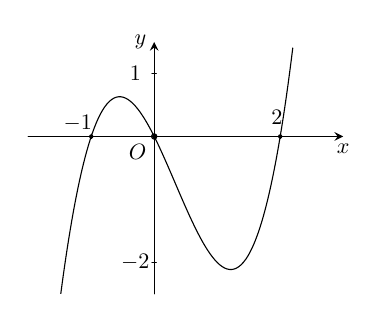
\begin{tikzpicture}[scale=0.8,line join=round, line cap=round,>=stealth]			
			\tikzset{every node/.style={scale=0.8}}  
			\def \xmin{-2}		\def \xmax{3}
			\def \ymin{-2.5}	\def \ymax{1.5}
			\def \ha{1*(\x)*((\x)+1)*((\x)-2)}		
			\draw[->] (\xmin,0)--(\xmax,0) node[below] {$x$};
			\draw[->] (0,\ymin)--(0,\ymax) node[left] {$y$};
			\draw (0,0)circle (1.2pt) node [below left] {$O$};
			\foreach \x/\g in {-1/135,2/100}
			\draw[thin] (\x,1pt)--(\x,-1pt) (\x,0) node [shift={(\g:0.3)}] {$\x$};			
			\foreach \y/\g in {-2/180,1/180}
			\draw[thin] (1pt,\y)--(-1pt,\y) (0,\y) node [shift={(\g:0.3)}]  {$\y$};				
			\begin{scope}
				\clip (\xmin+0.01,\ymin+0.01) rectangle (\xmax-0.01,\ymax-0.01);
				\draw[samples=100,domain=-1.5:2.2,smooth,variable=\x] plot (\x,{\ha});
			\end{scope}
			\foreach \x/\y in {-1/0,0/0,2/0}
			\fill[black] (\x,\y) circle(1pt); %%tô điểm		
		\end{tikzpicture}
	}
	\loigiai{
		Dựa vào đồ thị hàm số $y=f'(x)$, ta thấy
		\begin{itemize}
			\item $f'(x) > 0$ trên khoảng $(-1; 0)$ và $(2; +\infty)$.
			\item $f'(x) < 0$ trên khoảng $(-\infty; -1)$ và $(0; 2)$.
		\end{itemize}
		Hàm số $y=f(x)$ đồng biến trên các khoảng mà $f'(x) > 0$.\\
		Vậy hàm số đồng biến trên khoảng $(-1; 0)$.
	}
\end{ex}

%%%=============EX_8=============%%%
\begin{ex}%[Dự án đề TT THPTQG2026]%[2D1H1-2]
	Tính đạo hàm của hàm số $y=\mathrm{e}^x+\log x$.
	\choice
	{$y'=\mathrm{e}^x-\dfrac{1}{x\ln 10}$}
	{$y'=\mathrm{e}^x+\dfrac{1}{x}$}
	{\True $y'=\mathrm{e}^x+\dfrac{1}{x\ln 10}$}
	{$y'=\mathrm{e}^x-\dfrac{1}{x}$}
	\loigiai{		
		Ta có $y=\mathrm{e}^x+\log x$ suy ra $y'=\mathrm{e}^x+\dfrac{1}{x\ln 10}$.
	}
\end{ex}

%%%=============EX_9=============%%%
\begin{ex}%[Dự án đề TT THPTQG2026]%[2D1H2-2]
	\immini{
	Cho hàm số $y=f(x)$ xác định, có đạo hàm trên $\mathbb{R}$ và có bảng biến thiên như sau.
	Giá trị cực đại của hàm số bằng
	\choice
	{$-2$}
	{$0$}
	{$-3$}
	{\True $1$}
	}{
		
\begin{tikzpicture}
			\tkzTabInit[lgt=1.2,espcl=1.7,deltacl=0.6]
			{$x$/0.7,$y'$ /0.7,$y$ /1.5}
			{$-\infty$,$-2$,$0$,$+\infty$}
			\tkzTabLine{,+,0,-,0,+,}
			\tkzTabVar{-/$-\infty$,+/$1$,-/$-3$,+/$+\infty$}
		\end{tikzpicture}
	}
	\loigiai{
		Dựa vào bảng biến thiên, hàm số đạt cực đại tại $x=-2$ và giá trị cực đại là $y_{\text{CĐ}} = 1$.
	}
\end{ex}

%%%=============EX_10=============%%%
\begin{ex}%[Dự án đề TT THPTQG2026]%[0D8N2-4]
	Có bao nhiêu cách chọn $3$ học sinh từ $10$ học sinh?
	\choice
	{$\mathrm {A}_{10}^3$}
	{$10^3$}
	{$3^{10}$}
	{\True $\mathrm {C}_{10}^3$}
	\loigiai{
		Số cách chọn $3$ học sinh từ $10$ học sinh là $\mathrm {C}_{10}^3$.
	}
\end{ex}

%%%=============EX_11=============%%%
\begin{ex}%[Dự án đề TT THPTQG2026]%[2D3H1-3]
	Khảo sát thời gian tập thể dục của một số học sinh thu được mẫu số liệu ghép nhóm như sau:
	\begin{center}
		\begin{tabular}{|c|c|c|c|c|c|c|}
			\hline
			Thời gian (phút) & $[0;10)$ & $[10;20)$ & $[20;30)$ & $[30;40)$ & $[40;50)$ & $[50;60)$ \\ \hline
			Số học sinh & $10$ & $15$ & $22$ & $26$ & $20$ & $17$ \\ \hline
		\end{tabular}
	\end{center}
	Tìm trung vị của mẫu số liệu trên (\textit{làm tròn kết quả đến hàng phần mười}).
	\choice
	{$32,2$}
	{$31,4$}
	{\True $33,1$}
	{$33,2$}
	\loigiai{
		Tổng số học sinh $n = 10+15+22+26+20+17 = 110$.\\
		Vị trí trung vị là $\dfrac{n}{2} = 55$ suy ra trung vị thuộc nhóm $[30; 40)$.\\ 
		Vậy trung vị mẫu số liệu trên là		
		\[M_e = 30 + \dfrac{55 - 47}{26} \cdot 10 = 30 + \dfrac{8}{26} \cdot 10 = 30 + \dfrac{80}{26} \approx 33,1.\]
	}
\end{ex}

%%%=============EX_12=============%%%
\begin{ex}%[Dự án đề TT THPTQG2026]%[2H2N1-2]
	\immini[thm]{
		Cho hình hộp $ABCD.A'B'C'D'$. Khẳng định nào sau đây là đúng?
		\choice
		{$\overrightarrow{AB}+\overrightarrow{AD}+\overrightarrow{AA'}=\overrightarrow{AC}$}
		{$\overrightarrow{AB}+\overrightarrow{AD}+\overrightarrow{AA'}=\overrightarrow{AB'}$}
		{$\overrightarrow{AB}+\overrightarrow{AD}+\overrightarrow{AA'}=\overrightarrow{AD'}$}
		{\True $\overrightarrow{AB}+\overrightarrow{AD}+\overrightarrow{AA'}=\overrightarrow{AC'}$}
	}{
		\begin{tikzpicture}[scale=0.4, font=\footnotesize,line join=round, line cap=round, >=stealth]
			\path 
			(0,0) coordinate (A)
			++(-130:3) coordinate (B)
			++(0:4) coordinate (C)
			($(A)+(C)-(B)$) coordinate (D)
			($(A)!1/2!(C)$) coordinate (O)
			;
			\foreach \i in {A,B,C,D}{
				\coordinate (\i') at ($(\i)+(0,4)$);
			}
			\draw (A')--(B')--(C')--(D')--cycle;
			\draw (B)--(B') (C)--(C') (D)--(D')  (B)--(C)--(D);
			\draw[dashed,thin](B)--(A)--(A') (A)--(D);			
			\foreach \i/\g in {A'/90,B'/90,C'/90,D'/90,A/-90,B/-90,C/-90,D/-90}
			\fill[black] (\i) circle(1pt)+(\g:5mm)node[scale=1]{$\i$};
		\end{tikzpicture}
	}
	\loigiai{
		\immini {
			Theo quy tắc hình hộp, ta có $\overrightarrow{AB}+\overrightarrow{AD}+\overrightarrow{AA'}=\overrightarrow{AC}+\overrightarrow{AA'}=\overrightarrow{AC'}$.
		}{
			\begin{tikzpicture}[scale=0.4, font=\footnotesize,line join=round, line cap=round, >=stealth]
				\path 
				(0,0) coordinate (A)
				++(-130:3) coordinate (B)
				++(0:4) coordinate (C)
				($(A)+(C)-(B)$) coordinate (D)
				($(A)!1/2!(C)$) coordinate (O)
				;
				\foreach \i in {A,B,C,D}{
					\coordinate (\i') at ($(\i)+(0,4)$);
				}
				\draw (A')--(B')--(C')--(D')--cycle;
				\draw (B)--(B') (C)--(C') (D)--(D')  (B)--(C)--(D);
				\draw [dashed,->](A)--(B);
				\draw[dashed,->](A)--(D);
				\draw[dashed,->](A)--(A');				
				\draw[dashed,->](A)--(C');	
				\draw[dashed,->](A)--(C);					
				\foreach \i/\g in {A'/90,B'/90,C'/90,D'/90,A/180,B/-90,C/-90,D/-90}
				\fill[black] (\i) circle(1pt)+(\g:5mm)node[scale=1]{$\i$};
			\end{tikzpicture}
		}
	}
\end{ex}



\Closesolutionfile{ans}


\cauds
\Opensolutionfile{ans}[ans/ans-26-2--SoGD-L1-DS]



\begin{ex}%[Dự án đề TT THPTQG2026]%[2H2H2-4]
	Trong không gian với hệ tọa độ $Oxyz$, cho tam giác $ABC$, với $A(5;1;3)$, $B(1;6;2)$, $C(5;0;4)$.
	\choiceTF
	{$\overrightarrow{AB}=(-4;5;-1)$, $\overrightarrow{AC}=(0;-1;-1)$}
	{\True Biết điểm $D(a;b;c)$ sao cho tứ giác $ABCD$ là hình bình hành, ta có $a+b+c=9$}
	{$\overrightarrow{AB}\cdot\overrightarrow{AC}=-10$}
	{Gọi $\alpha$ là số đo góc $A$ của tam giác $ABC$. Khi đó $\cos \alpha = \dfrac{\sqrt{21}}{7}$}
	\loigiai{
		\begin{itemchoice}
			\itemch Ta có 
			\begin{itemize}
				\item $\overrightarrow{AB} = (1-5; 6-1; 2-3) = (-4; 5; -1)$;
				\item $\overrightarrow{AC} = (5-5; 0-1; 4-3) = (0; -1; 1)$.
			\end{itemize}
			\itemch Tứ giác $ABCD$ là hình bình hành khi và chỉ khi
			\[\overrightarrow{AB} = \overrightarrow{DC}\Leftrightarrow \heva{&5-a=-4 \\ &-b=5 \\ &4-c=-1} \Rightarrow \heva{&a=9\\&b=-5\\&c=5.}\]
			Khi đó $a+b+c = 9 + (-5) + 5 = 9$.		
			\itemch Ta có $\overrightarrow{AB} \cdot \overrightarrow{AC} = (-4) \cdot 0 + 5 \cdot (-1) + (-1) \cdot 1 = 0 - 5 - 1 = -6$.
			\itemch Ta có 
			\begin{itemize}
				\item $\left| \overrightarrow{AB}\right|  = \sqrt{(-4)^2 + 5^2 + (-1)^2}= \sqrt{42}$;
				\item $\left| \overrightarrow{AC}\right|  = \sqrt{0^2 + (-1)^2 + 1^2} = \sqrt{2}$.
			\end{itemize} 
			Suy ra
			\[\cos \alpha = \cos \left( \overrightarrow{AB}, \overrightarrow{AC}\right)  = \dfrac{\overrightarrow{AB} \cdot \overrightarrow{AC}}{\left| \overrightarrow{AB}\right|  \cdot\left| \overrightarrow{AC}\right| }= \dfrac{-6}{\sqrt{42} \cdot \sqrt{2}} = -\dfrac{\sqrt{21}}{7}.\]
		\end{itemchoice}
	}
\end{ex}

%%%=============EX_2=============%%%
\begin{ex}%[Dự án đề TT THPTQG2026]%[2D1H3-1]
	Cho hàm số $f(x)=x-\ln x$. Khi đó
	\choiceTF
	{\True Tập xác định của hàm số là  $\mathscr {D}=(0;+\infty)$}
	{\True Đạo hàm $f'(x)=1-\dfrac{1}{x}$}
	{\True Phương trình $f'(x)=0$ có nghiệm duy nhất $x=1$}
	{\True Giá trị lớn nhất của hàm số $f(x)$ trên đoạn $\left[ \dfrac{1}{3}; 2\right] $ bằng $\dfrac{1}{3}+\ln 3$}
	\loigiai{
		\begin{itemchoice}
			\itemch Điều kiện xác định $x > 0$.\\ 
			Tập xác định $\mathscr{D}=(0;+\infty)$.
			\itemch Ta có $f'(x) = (x - \ln x)' = 1 - \dfrac{1}{x}$.
			\itemch Xét $f'(x) = 0 \Leftrightarrow 1 - \dfrac{1}{x} = 0 \Leftrightarrow x = 1$ (thoả mãn điều kiện).\\
			Vậy phương trình $f'(x)=0$ có nghiệm duy nhất $x=1$.
			\itemch Xét hàm số $f(x)$ trên đoạn $\left[ \dfrac{1}{3}; 2\right] $ .\\
			Ta có $f(1) = 1 - \ln 1 = 1$;	$f\left( \dfrac{1}{3}\right)  = \dfrac{1}{3} +\ln 3$; $f(2) = 2 - \ln 2$.\\			
			Vậy giá trị lớn nhất của hàm số $f(x)$ trên đoạn $\left[ \dfrac{1}{3}; 2\right] $ bằng $\dfrac{1}{3} + \ln 3$.
		\end{itemchoice}
	}
\end{ex}

%%%=============EX_3=============%%%
\begin{ex}%[Dự án đề TT THPTQG2026]%[2D1H3-6]
	Một xưởng mộc dùng gỗ sồi để sản xuất $5$ chiếc bàn mỗi ngày. Chi phí cho mỗi lần vận chuyển nguyên liệu là $5\,625$ USD, chi phí để lưu trữ một đơn vị nguyên liệu là $10$ USD mỗi ngày. Giả sử lượng nguyên liệu cần thiết để sản xuất một chiếc bàn là $1$ đơn vị và lưu ý rằng trong mỗi ngày của chu kì sản xuất (thời gian giữa hai lần nhập nguyên liệu liên tiếp) thì lượng nguyên liệu lưu trữ trung bình mỗi ngày được tính bằng một nửa tổng lượng nguyên liệu tồn kho đầu kì và lượng nguyên liệu tồn kho cuối kì. Giả sử nguyên liệu được nhập về sau mỗi $x$ ngày.
	\choiceTF
	{\True Một chu kì sản xuất, xưởng mộc này nhập về $5x$ đơn vị nguyên liệu}
	{Chi phí để lưu trữ nguyên liệu trong $x$ ngày của một chu kì sản xuất là $50x^2$ USD}
	{Hàm chi phí trung bình mỗi ngày trong một chu kì sản xuất là $c(x) = 50x + \dfrac{5\,625}{x}$}
	{\True Để chi phí trung bình mỗi ngày là một chu kì sản xuất là ít nhất thì xưởng mộc nên nhập hàng sau mỗi $15$ ngày và mỗi lần nhập về $75$ đơn vị nguyên liệu}
	\loigiai{
		\begin{itemchoice}
			\itemch Mỗi ngày sản xuất $5$ chiếc bàn, mỗi chiếc cần $1$ đơn vị nguyên liệu.\\ 
			Vậy mỗi ngày tiêu thụ $5$ đơn vị nguyên liệu.\\
			Chu kì sản xuất là $x$ ngày, nên tổng số nguyên liệu cần nhập là $5x$ đơn vị.
			\itemch Lượng nguyên liệu tồn kho đầu kì là $5x$ (nhập về).\\ 
			Lượng tồn kho cuối kì là $0$ (dùng hết sau $x$ ngày).\\
			Lượng nguyên liệu lưu trữ trung bình mỗi ngày là $\dfrac{5x + 0}{2} = \dfrac{5x}{2}$.\\
			Chi phí lưu trữ mỗi ngày cho một đơn vị là $10$ USD.\\ 
			Vậy chi phí lưu trữ trung bình mỗi ngày là $10 \cdot \dfrac{5x}{2} = 25x$ USD.\\
			Tổng chi phí lưu trữ trong $x$ ngày là $25x \cdot x = 25x^2$ USD.
			\itemch Tổng chi phí cho một chu kì $x$ ngày gồm chi phí vận chuyển và chi phí lưu trữ
			\[C(x) = 5\,625 + 25x^2.\]
			Chi phí trung bình mỗi ngày là
			$p(x) = \dfrac{C(x)}{x} = \dfrac{5\,625 + 25x^2}{x} = \dfrac{5\,625}{x} + 25x$.			
			\itemch Để chi phí trung bình mỗi ngày thấp nhất, áp dụng bất đẳng thức AM-GM cho hai số dương
			\[p(x) \ge 2\sqrt{25x \cdot \dfrac{5\,625}{x}} = 2\sqrt{25 \cdot 5\,625} = 750.\]
			Đẳng thức xảy ra khi $25x = \dfrac{5\,625}{x} \Leftrightarrow x^2 = \dfrac{5\,625}{25} = 225 \Leftrightarrow x = 15$.\\
			Vậy xưởng nên nhập hàng sau mỗi $15$ ngày.\\
			Lượng hàng nhập về mỗi lần là $5x = 5 \cdot 15 = 75$ đơn vị nguyên liệu.
		\end{itemchoice}
	}
\end{ex}

%%%=============EX_4=============%%%
\begin{ex}%[Dự án đề TT THPTQG2026]%[1H8V6-6]
	Cho hình lăng trụ $ABC.A'B'C'$ có tam giác $ABC$ vuông cân tại $A$, hình chiếu vuông góc $H$ của $A'$ trên mặt phẳng $(ABC)$ trùng với trọng tâm tam giác $ABC$. Biết $AA'=BC=2a$.
	\choiceTF
	{\True Độ dài đường cao hình lăng trụ bằng $\dfrac{4a\sqrt{2}}{3}$}
	{Thể tích khối lăng trụ đã cho bằng $4a^3\sqrt{2}$}
	{\True Khoảng cách giữa hai đường thẳng $BB'$ và $AC$ gấp ba lần khoảng cách từ $H$ đến $(ACC'A')$}
	{Khoảng cách giữa hai đường thẳng $BB'$ và $AC$ bằng $\dfrac{2a\sqrt{34}}{17}$}
	\loigiai{
		\begin{center}
			\begin{tikzpicture}[scale=1, font=\footnotesize, line join=round, line cap=round]				
				% --- 1. Thiết lập tọa độ ---	
				\coordinate (A) at (0,0);
				\coordinate (B) at (1.5, -1.5);
				\coordinate (C) at (4, 0);
				\coordinate (M) at ($(B)!0.5!(C)$);
				\coordinate (H) at (barycentric cs:A=1,B=1,C=1);
				\coordinate (A') at ($(H)+(0, 3)$);
				\coordinate (vecAA) at ($(A')-(A)$);
				\coordinate (B') at ($(B)+(vecAA)$);
				\coordinate (C') at ($(C)+(vecAA)$);
				\coordinate (P) at ($(A)!0.5!(C)$);
				\coordinate (K) at ($(A)!2/3!(P)$);
				% --- 2. Vẽ hình ---
				\draw[dashed] (A') -- (H) (A) -- (C) (A) -- (B) (A) -- (H) (A) -- (M); 			
				\draw[dashed] (A) -- (C)  (A) -- (B)  (A) -- (A') (A') -- (H)  (B) -- (P) (H) -- (K)--(A')  ;	
				\draw (B) -- (C) (B) -- (B') (C) -- (C') (A') -- (B') (B') -- (C') (C') -- (A') (A) -- (A') (A) -- (B)
				(B) -- (C) (B) -- (B') (C) -- (C')  (B') -- (C') (C') -- (A') (A') -- (B');
				
				% --- 3. Ký hiệu và Điểm ---
				\foreach \i/\g in {A/180,B/-90,C/0,A'/90,B'/90,C'/90,H/-135,M/-30,P/60,K/135}
				\fill[black] (\i) circle(1pt)+(\g:2.5mm)node[scale=1]{$\i$};
				\foreach \a/\b/\c in {A'/H/M,B/A/C,H/K/A,A'/K/C}{\draw pic[draw,angle radius=2mm] {right angle = \a--\b--\c};}				
				% Ký hiệu trung điểm M
				\node[font=\tiny] at ($(B)!0.5!(M)$) {/};
				\node[font=\tiny] at ($(M)!0.5!(C)$) {/};				
			\end{tikzpicture}
		\end{center}
		\begin{itemchoice}
			\itemch Tam giác $ABC$ vuông cân tại $A$, $BC=2a \Rightarrow AB=AC=a\sqrt{2}$.\\
			Trung tuyến $AM = \dfrac{1}{2}BC = a$.\\
			Trọng tâm $H$ thuộc $AM$ và $AH = \dfrac{2}{3}AM = \dfrac{2a}{3}$.\\
			Tam giác $A'HA$ vuông tại $H$ có đường cao lăng trụ là $A'H$ là
			\[A'H = \sqrt{AA'^2 - AH^2} = \sqrt{(2a)^2 - \left( \dfrac{2a}{3}\right) ^2} = \dfrac{4a\sqrt{2}}{3}.\]			 
			\itemch Diện tích đáy $S_{ABC} = \dfrac{1}{2}AB \cdot AC = \dfrac{1}{2} \cdot a\sqrt{2} \cdot a\sqrt{2} = a^2$.\\
			Thể tích $V = S_{ABC} \cdot A'H = a^2 \cdot \dfrac{4a\sqrt{2}}{3} = \dfrac{4a^3\sqrt{2}}{3}$.		
			\itemch Gọi $P=BH\cap AC$ suy ra $P$ là trung điểm $AC$. Khi đó			
			\[\dfrac{\mathrm {d}\big(B, (ACC'A')\big)}{\mathrm {d}\big(H, (ACC'A')\big) } =\dfrac{BP}{HP} = 3.\]
			\itemch Tính $\mathrm {d}\big(BB', AC\big) = \mathrm {d}\big(B, (ACC'A')\big)$.\\
			Ta có
			\begin{itemize}
				\item $V_{B.ACC'A'} = \dfrac{1}{3} \mathrm {d}(B, (ACC'A')) \cdot S_{ACC'A'}$;
				\item $V_{B.ACC'A'} =2 V_{A'.ABC}$;
				\item $V_{A'.ABC} = \dfrac{1}{3} A'H \cdot S_{ABC} = \dfrac{1}{3} \cdot \dfrac{4a\sqrt{2}}{3} \cdot a^2 = \dfrac{4a^3\sqrt{2}}{9}$.
			\end{itemize} 
			$K$ là chân đường cao hạ từ $H$ xuống $AC$.\\
			Trong $\Delta ABC$ vuông cân tại $A$ có $H$ trọng tâm.\\
			$K$ nằm trên $AC$ và $HK \parallel AB$ suy ra $HK = \dfrac{1}{3} AB = \dfrac{a\sqrt{2}}{3}$.\\
			Đường cao của hình bình hành $ACC'A'$ ứng với cạnh $AC$ là đoạn $A'K$.\\
			$A'K = \sqrt{A'H^2 + HK^2} = \sqrt{\dfrac{32a^2}{9} + \dfrac{2a^2}{9}} = \sqrt{\dfrac{34a^2}{9}} = \dfrac{a\sqrt{34}}{3}$.\\
			$S_{ACC'A'} = AC \cdot A'K = a\sqrt{2} \cdot \dfrac{a\sqrt{34}}{3} = \dfrac{2a^2\sqrt{17}}{3}$.\\
			Suy ra 			
			\[\mathrm {d}\big(B, (ACC'A')\big) = \dfrac{3 V_{B.ACC'A'}}{S_{ACC'A'}} = \dfrac{3 \cdot \dfrac{2\cdot4a^3\sqrt{2}}{9}}{\dfrac{2a^2\sqrt{17}}{3}} = \dfrac{4a\sqrt{2}}{\sqrt{17}} = \dfrac{4a\sqrt{34}}{17}.\]			
		\end{itemchoice}
	}
\end{ex}



\Closesolutionfile{ans}

\caukq
\Opensolutionfile{ans}[ans/ans-26-2--SoGD-L1-KQ]



\begin{ex}%[Dự án đề TT THPTQG2026]%[1H8V7-2]
	Cho tứ diện đều $ABCD$ có cạnh bằng $1$. Trên các mặt phẳng $(BCD)$, $(CDA)$, $(DAB)$, $(ABC)$ lần lượt lấy các điểm $A_1$, $B_1$, $C_1$, $D_1$ sao cho các đường thẳng $A_1B_1$, $B_1C_1$, $C_1D_1$, $D_1A_1$ lần lượt vuông góc với các mặt phẳng $(BCD)$, $(CDA)$, $(DAB)$, $(ABC)$. Biết thể tích khối tứ diện $A_1B_1C_1D_1$ bằng $\dfrac{a}{b}\sqrt{2}$ với $a$, $b$ là các số nguyên dương và phân số $\dfrac{a}{b}$ tối giản. Tính $a+b$.
	\par
	%\shortans[0]{163}
	\loigiai{
		Gọi $O$ là trọng tâm của tứ diện đều $ABCD$.\\
		Theo giả thiết, ta có $OA \perp (BCD)$.\\
		Nên $OA \parallel A_1B_1 \Rightarrow \overrightarrow{A_1B_1} = k_1 \overrightarrow{OA}$.\\
		Tương tự $\heva{&\overrightarrow{B_1C_1} = k_2 \overrightarrow{OB}\\ &\overrightarrow{C_1D_1} = k_3 \overrightarrow{OC}\\ &\overrightarrow{D_1A_1} = k_4 \overrightarrow{OD}.}$	\\	
		Ta có $\overrightarrow{A_1B_1} + \overrightarrow{B_1C_1} + \overrightarrow{C_1D_1} + \overrightarrow{D_1A_1} = \overrightarrow{0} \Leftrightarrow k_1 \overrightarrow{OA} + k_2 \overrightarrow{OB} + k_3 \overrightarrow{OC} + k_4 \overrightarrow{OD} = \overrightarrow{0}$.\\	
		Vì $O$ là trọng tâm của tứ diện $ABCD$ nên suy ra $\overrightarrow{OA} + \overrightarrow{OB} + \overrightarrow{OC} + \overrightarrow{OD} = \overrightarrow{0}$.\\
		Hay $k_1 \overrightarrow{OA} + k_1 \overrightarrow{OB} + k_1 \overrightarrow{OC} + k_1 \overrightarrow{OD} = \overrightarrow{0}\Rightarrow (k_1 - k_2) \overrightarrow{OB} + (k_1 - k_3) \overrightarrow{OC} + (k_1 - k_4) \overrightarrow{OD} = \overrightarrow{0} \quad (\ast)$.\\	
		Do các vectơ $\overrightarrow{OB}$, $\overrightarrow{OC}$ và $\overrightarrow{OD}$ không đồng phẳng nên $(\ast) \Leftrightarrow k_1 = k_2 = k_3 = k_4 = k$.\\	
		\immini{
			Chọn hệ trục tọa độ $Oxyz$ sao cho $A(1; 1; 1)$, $B(1; -1; -1)$, $C(-1; 1; -1)$ và $D(-1; -1; 1)$.\\
			Khi đó $AB = BC = CD = DA = AC = BD = 2\sqrt{2}$.\\
			Vì tứ diện $ABCD$ có cạnh bằng $1$ nên $1$ đơn vị trên trục bằng $2\sqrt{2}$ đơn vị độ dài.\\
			Ta có
			\begin{itemize}
				\item $(BCD)\colon x + y + z + 1 = 0$;
				\item $(CDA)\colon x - y - z + 1 = 0$;
				\item $(DAB)\colon -x + y - z + 1 = 0$;
				\item $(ABC)\colon -x - y + z + 1 = 0$.
			\end{itemize}	
			Gọi $A_1(x; y; z)$.\\
			Vì $\overrightarrow{A_1B_1} = k \overrightarrow{OA} \Rightarrow B_1(x+k; y+k; z+k)$.\\
			Tương tự $C_1(x+2k; y; z)$ và $D_1(x+k; y+k; z-k)$.\\	
		}{
			\tdplotsetmaincoords{70}{-40}
			\begin{tikzpicture}[tdplot_main_coords, scale=2.3, line join=round, line cap=round,>=stealth]	
				% 1. Vẽ hệ trục tọa độ Oxyz
				\draw[->, blue, thick] (-1.5,0,0) -- (1.8,0,0) node[right] {$x$};
				\draw[->, blue, thick] (0,-1.5,0) -- (0,1.8,0) node[above] {$y$};
				\draw[->, blue, thick] (0,0,-1.5) -- (0,0,1.8) node[left] {$z$};
				\node[below left] at (0,0,0) {$O$};	
				% 2. Định nghĩa tọa độ các đỉnh ABCD
				\coordinate (A) at (1,1,1);
				\coordinate (B) at (1,-1,-1);
				\coordinate (C) at (-1,1,-1);
				\coordinate (D) at (-1,-1,1);	
				% 3. Định nghĩa tọa độ các đỉnh A1, B1, C1, D1
				\coordinate (A1) at (-2/3, -1/3, 0);
				\coordinate (B1) at (0, 1/3, 2/3);
				\coordinate (C1) at (2/3, -1/3, 0);
				\coordinate (D1) at (0, 1/3, -2/3);	
				% 4. Vẽ các cạnh
				\draw[dashed, gray!60] (B) -- (C) (C) -- (D) (B) -- (D)  (A) -- (D);		
				\draw[thick, black] (A) -- (B)  (A) -- (C)--(B) ;	
				% 5. Vẽ tứ diện nội tiếp A1B1C1D1 
				\fill[red!20, opacity=0.5] (A1) -- (B1) -- (C1) -- cycle;	
				\draw[red, thick, dashed] (A1) -- (B1) -- (C1) -- (D1) -- cycle (A1) -- (C1) (B1) -- (D1) (A1) -- (D1); 	
				% 7. Đánh dấu các điểm
				\foreach \p/\pos in {A/above, B/right, C/left, D/below} {
					\fill[black] (\p) circle (0.5pt);
					\node[\pos, font=\footnotesize] at (\p) {$\p$};
				}	
				\foreach \p/\pos/\name in {A1/left/A_1, B1/above right/B_1, C1/below/C_1, D1/below/D_1} {
					\fill[red] (\p) circle (0.5pt);
					\node[\pos, red] at (\p) {$\name$};
				}	
			\end{tikzpicture}
		} \noindent
		Ta có hệ
		$\heva{
			&x + y + z + 1 = 0 \\
			&x + k - (y + k) - (z + k) + 1 = 0 \\
			&-(x + 2k) + y - k + 1 = 0 \\
			&-(x + k) - (y + k) + z - k + 1 = 0
		}
		\Leftrightarrow
		\heva{
			&x = - \dfrac{2}{3} \\
			&y = - \dfrac{1}{3} \\
			&z = 0 \\
			&k = \dfrac{2}{3}.
		}$\\
		Vậy $\overrightarrow{A_1B_1} = \left( \dfrac{2}{3}; \dfrac{2}{3}; \dfrac{2}{3} \right)$, $\overrightarrow{B_1C_1} = \left( \dfrac{2}{3}; -\dfrac{2}{3}; -\dfrac{2}{3} \right)$ và $\overrightarrow{C_1D_1} = \left( -\dfrac{2}{3}; \dfrac{2}{3}; -\dfrac{2}{3} \right)$.\\
		Thể tích khối tứ diện $A_1B_1C_1D_1$ trong hệ tọa độ đã chọn
		\[V' = \dfrac{1}{6} \left| \left[ \overrightarrow{A_1B_1}, \overrightarrow{A_1C_1}\right]  \cdot \overrightarrow{A_1D_1} \right|= \dfrac{1}{6}\left[ 0 \cdot \dfrac{2}{3} + \dfrac{8}{9} \cdot \dfrac{2}{3} + \left(-\dfrac{8}{9}\right) \cdot \left(-\dfrac{2}{3}\right)\right]  = \dfrac{1}{6} \cdot \dfrac{32}{27} = \dfrac{16}{81}. \]	
		Tỉ lệ độ dài là $L = \dfrac{1}{2\sqrt{2}}$.\\
		Thể tích thật $V = V' \cdot L^3 = \dfrac{16}{81} \cdot \left(\dfrac{1}{2\sqrt{2}}\right)^3 = \dfrac{1}{81\sqrt{2}} = \dfrac{\sqrt{2}}{162}$.\\
		Ta có $V = \dfrac{a}{b}\sqrt{2} = \dfrac{1}{162}\sqrt{2} \Rightarrow a=1$, $b=162$.\\
		Vậy $a+b = 1+162 = 163$.
	}
\end{ex}
%%%=============BT_2=============%%%
\begin{ex}%[Dự án đề TT THPTQG2026]%[1H8V7-9]
	\immini[thm]{
		Anh A mở một nhà hàng lẩu. Anh đã trang bị cho mỗi bàn ăn một nồi lẩu có dạng hình trụ dọc, bán kính đáy nồi (ngoài) là $R=15$ cm, bán kính trụ giữa (trong) là $r=3{,}5$ cm, chiều cao nồi là $h=10$ cm. Để khách hàng có trải nghiệm tốt nhất, anh A cần xác định chiều dài tối thiểu của chiếc đũa sao cho dù đầu đũa có bị trượt vào vị trí nào trong nồi, phần đầu đũa thừa ra ngoài miệng nồi vẫn phải lớn hơn $5$ cm. Tính $L$ (\textit{làm tròn kết quả đến phần mười}).
	}{
		\begin{tikzpicture}[scale=0.15, font=\sffamily\scriptsize,line join=round, line cap=round,>=stealth]	
			% --- THÔNG SỐ ---
			\def\R{15}   % Bán kính ngoài
			\def\r{3.5}  % Bán kính trong
			\def\H{10}   % Chiều cao nồi
			\def\WaterH{7} % Mực nước			
			% --- 1. VẼ NỀN VÀ ĐÁY NỒI ---
			% Đáy nồi (Kim loại đáy)
			\fill[gray!30] (0,0) ellipse ({\R} and 4);
			\draw[gray!80, thick] (-\R,0) arc (180:360:\R cm and 4cm);
			\draw[gray!50, dashed] (-\R,0) arc (180:0:\R cm and 4cm);			
			% --- 2. VẼ TRỤ GIỮA (ỐNG NHIỆT) ---
			% Thân trụ giữa (Gradient xám kim loại)
			\shade[left color=gray!40, right color=gray!10, middle color=white] 
			(-\r,0) -- (-\r,\H) arc (180:0:\r cm and 1cm) -- (\r,0) arc (360:180:\r cm and 1cm);	
			% Viền trụ giữa
			\draw[gray!80] (-\r,0) -- (-\r,\H);
			\draw[gray!80] (\r,0) -- (\r,\H);
			\draw[gray!80, dashed] (-\r,0) arc (180:0:\r cm and 1cm); % Đáy trụ khuất
			\draw[gray!80] (-\r,0) arc (180:360:\r cm and 1cm);	
			% Miệng trụ giữa
			\fill[gray!20] (0,\H) ellipse ({\r} and 1);
			\draw[gray!80] (0,\H) ellipse ({\r} and 1);		
			% Miệng nồi
			\draw[thick, gray!80] (0,\H) ellipse ({\R} and 4);	
			% Mực nước (Viền mặt thoáng)
			\draw[orange!80!red, thin] (0,\WaterH) ellipse ({\R} and 4);
			% --- 5. VẼ ĐÔI ĐŨA (GỖ 3D) ---
			% Đũa 1: Cắm nghiêng
			\def\StickW{0.4} % Độ dày đũa
			\coordinate (A1) at (6, 0.5); % Chân đũa
			\coordinate (B1) at (14, \H + 1); % Điểm tựa
			
			% Vẽ thân đũa (Hình chữ nhật dài nghiêng)
			\filldraw[fill=brown!80!black, draw=brown!40!black] 
			($(A1)+(-\StickW,0)$) -- ($(B1)+(-\StickW, \StickW)$) -- ($(B1)+(\StickW, \StickW)$) -- ($(A1)+(\StickW,0)$) -- cycle;			
			% Phần thừa ra (màu sáng hơn chút hoặc giống)
			\coordinate (C1) at ($(B1)!-5cm!(A1)$); % Kéo dài 5cm (tỉ lệ)
			\filldraw[fill=brown!80!black, draw=brown!40!black] 
			($(B1)+(-\StickW, \StickW)$) -- ($(C1)+(-\StickW, \StickW)$) -- ($(C1)+(\StickW, \StickW)$) -- ($(B1)+(\StickW, \StickW)$) -- cycle;	
			% Đũa 2 (Song song)
			\coordinate (A2) at ($(A1)+(1.5, -0.5)$);
			\coordinate (B2) at ($(B1)+(1.5, -0.5)$);
			\coordinate (C2) at ($(C1)+(1.5, -0.5)$);	
			\filldraw[fill=brown!80!black, draw=brown!40!black] 
			($(A2)+(-\StickW,0)$) -- ($(C2)+(-\StickW, \StickW)$) -- ($(C2)+(\StickW, \StickW)$) -- ($(A2)+(\StickW,0)$) -- cycle;		
			% --- 3. VẼ NƯỚC LẨU (SINH ĐỘNG) ---	
			% Vùng nước bao quanh trụ giữa (Cắt bỏ phần trụ giữa)
			\begin{scope}
				\fill[orange!20!red, opacity=0.4] (-\R,0) -- (-\R,\WaterH) arc (180:360:\R cm and 4cm) -- (\R,0) arc (360:180:\R cm and 4cm);			
				\fill[orange!30!red, opacity=0.5] (0,\WaterH) ellipse ({\R} and 4);
			\end{scope}
			% --- 2. VẼ TRỤ GIỮA (ỐNG NHIỆT) ---
			% Thân trụ giữa (Gradient xám kim loại)
			\shade[left color=gray!40, right color=gray!10, middle color=white] 
			(-\r,\WaterH) -- (-\r,\H) arc (180:360:\r cm and 1cm) -- (\r,\WaterH) arc (360:180:\r cm and 1cm);			
			\draw[gray!80] (-\r,0) -- (-\r,\WaterH);
			\draw[gray!80] (\r,0) -- (\r,\WaterH);
			\draw[gray!80] (-\r,\WaterH) arc (180:360:\r cm and 1cm);
			% --- 4. VẼ THÂN NỒI (THỦY TINH/KIM LOẠI TRONG SUỐT) ---
			% Thân nồi
			\draw[thick, gray!80] (-\R,0) -- (-\R,\H);
			\draw[thick, gray!80] (\R,0) -- (\R,\H);		
			% --- 6. GHI CHÚ KÍCH THƯỚC (ĐẸP HƠN) ---
			\draw[<->, >=stealth, blue] (-\R-2, 0) -- (-\R-2, \H) node[midway, fill=white,inner sep=0pt,sloped] {$h=10$};
			\draw[gray, thin] (-\R,0) -- (-\R-2.5,0);
			\draw[gray, thin] (-\R,\H) -- (-\R-2.5,\H);
			
			\draw[<->, >=stealth, blue] (0, -5) -- (\R, -5) node[midway, fill=white,inner sep=0pt,sloped] {$R=15$};
			\draw[gray, thin] (0,0) -- (0,-5.5);
			\draw[gray, thin] (\R,0) -- (\R,-5.5);
			
			\draw[<->, >=stealth, blue] (0, \H+2) -- (\r, \H+2) node[midway, ,inner sep=0pt,sloped,above] {$r=3{,}5$};
			\draw[gray, thin] (0,\H) -- (0,\H+2.5);
			\draw[gray, thin] (\r,\H) -- (\r,\H+2.5);	
			% Nhãn đũa L
			\draw[<->, >=stealth, red] ($(A2)+(2,0)$) -- node[midway, right] {$L$} ($(C2)+(2,0)$);	
		\end{tikzpicture}
	}
	\par
	%\shortans[0]{35,8}
	\loigiai{
		Hình chiếu vuông góc của chiếc đũa lên mặt đáy nồi là một dây cung của đường tròn bán kính $R$.\\
		Độ dài của dây cung này lớn nhất khi nó tiếp xúc với đường tròn đáy nhỏ bán kính $r$ và được tính bằng
		\[l = 2\sqrt{R^2 - r^2} = 2\sqrt{15^2 - 3{,}5^2} = 2\sqrt{212{,}75}\text{ (cm)}.\]
		Đường chéo lớn nhất của phần không gian chứa đũa trong nồi là cạnh huyền của tam giác vuông có hai cạnh góc vuông là $l$ và chiều cao $h$.
		\[L_{\text{trong}} = \sqrt{l^2 + h^2} = \sqrt{\left( 2\sqrt{212{,}75}\right) ^2 + 10^2}= \sqrt{951} \text{ (cm)}.\]
		Để phần thừa lớn hơn $5$ cm thì $L > L_{\text{trong}}+5= \sqrt{951}+5\approx 35{,}8$ cm.
	}
\end{ex}

%%%=============BT_3=============%%%
\begin{ex}%[Dự án đề TT THPTQG2026]%[0D8C2-5]
	Mèo Táo có mở một cửa hàng sách và đang cần tuyển nhân viên trông coi cửa hàng. Để tuyển nhân viên đòi hỏi có khả năng tư duy và suy luận tốt; Táo đưa ra thử thách như sau: Bộ truyện tranh thám tử Kenichi gồm $44$ tập đang được sắp xếp từ $1$ tới $44$ trên giá (giả sử đang tính từ trái qua phải và tất cả cuốn truyện được sắp xếp cùng chiều). Yêu cầu hãy thực hiện việc sắp xếp các tập truyện theo trình tự ngược lại từ $44$ tới $1$ theo quy tắc: đổi chỗ $2$ tập truyện đang xếp liên tiếp sẽ bị tính $1$ điểm; đổi chỗ $2$ tập truyện mà ở giữa chúng có $3$ tập khác thì không bị tính điểm. Bạn An muốn ứng tuyển vào nhân viên cửa hàng. Hỏi điểm số của An nhỏ nhất là bao nhiêu điểm để thực hiện được thử thách trên.
	\par
	%\shortans[0]{22}
	\loigiai{
		Một tập truyện $j$ ở \lq\lq vị trí tốt\rq\rq\ nếu nó ở vị trí thứ $i$ thỏa mãn ($i+j$) chia $4$ dư $1$.\\
		Ta có
		\begin{itemize}
			\item Cách đổi $0$ điểm không làm thay đổi số tập ở \lq\lq vị trí tốt\rq\rq.
			\item Cách đổi $1$ điểm thì làm tăng nhiều nhất $2$ tập ở \lq\lq vị trí tốt\rq\rq.
		\end{itemize}
		Ban đầu không có tập nào ở \lq\lq vị trí tốt\rq\rq\ để xếp được $44$ tập ở \lq\lq vị trí tốt\rq\rq.\\
		Yêu cầu bài toán cần thực hiện ít nhất $22$ cách đổi \lq\lq $1$ điểm\rq\rq.\\
		Ta thực hiện các bước đổi sau
		\begin{itemize}
			\item Bước $1$ đến $21$ đổi $i$ với $i+1$ với $i \in \{2; 4; 6; \dots; 42\}$ (bị tính $21$ điểm).
			\item Sau $21$ bước thì tất các tập ngoại trừ tập $1$ và $44$ đều ở \lq\lq vị trí tốt\rq\rq.
			\item Bước $22$ ta đổi tập $1$ và tập đang ở vị trí $5$ ($0$ điểm).
			\item Đổi tập $44$ và tập đang ở vị trí $40$ ($0$ điểm), sau đó cứ đổi theo quy luật từ vị trí $40$ về vị trí $36$, từ vị trí $36$ về vị trí $32$, \dots về vị trí $4$.
			\item Sau đó đổi tập $44$ ở vị trí $4$ đổi với tập $1$ ở vị trí $5$ ($1$ điểm).
		\end{itemize}
		Lúc này các tập đã ở \lq\lq vị trí tốt\rq\rq\ và ở các vị trí $1$, $5$, $\dots$, $41$ chỉ có các tập $4$, $8$, $\ldots$, $44$ ta có thể thực hiện các bước đổi $0$ điểm để các tập này sắp xếp theo thứ tự giảm dần.\\
		Vậy số điểm nhỏ nhất An thực hiện được là $22$ điểm.
	}
\end{ex}

%%%=============BT_4=============%%%
\begin{ex}%[Dự án đề TT THPTQG2026]%[2H5V3-4]
	Mặt cầu tâm $I$ bán kính $R>0$ là tập hợp tất cả các điểm trong không gian cách $I$ một khoảng bằng $R$. Trong không gian với hệ tọa độ $Oxyz$, đơn vị trên hệ trục là cm, một tổ kiến có bề mặt là một mặt cầu tâm là gốc tọa độ và bán kính $R=6$ cm, ở điểm $A(20;0;0)$ có $10$ miếng mồi và ở điểm $B(0;20;0)$ có $3$ miếng mồi. Một con kiến trên bề mặt tổ, mỗi lần đi đến $A$ hoặc $B$ tha đúng một miếng mồi về tổ. Hỏi quãng đường ngắn nhất con kiến đó đi là bao nhiêu cm để con kiến tha hết $13$ miếng mồi về tổ (\textit{làm tròn kết quả hàng đơn vị})?
	\par
	%\shortans[0]{369}
	\loigiai{
		\immini{
			Dễ thấy, $A(20; 0; 0)$ và $B(0; 20; 0)$ đều thuộc mặt phẳng $(Oxy)$ nên đường đi ngắn nhất từ một điểm trên mặt cầu đến $A$ (hoặc $B$) nằm trong mặt phẳng $(Oxy)$.\\
			Đưa bài toán về hệ tọa độ $Oxy$ với đường tròn tâm $O$, bán kính $6$ cm và $A(20; 0)$; $B(0; 20)$.\\
			Để tổng quãng đường ngắn nhất, con kiến phải xuất phát và trở về mặt tổ tại điểm trên mặt cầu gần $A$ và $B$ nhất, lần lượt là các điểm $M(6; 0)$ và $N(0; 6)$.\\
			Giả sử, con kiến sẽ lần lượt lấy các miếng mồi ở $A$ rồi đến các miếng mồi ở $B$.\\ Tuy nhiên, khi lấy miếng mồi thứ $10$ ở $A$, con kiến sẽ về một điểm khác trên mặt tổ thay vì quay về $M$ rồi đi theo đường cung tròn $MN$ để đến $N$.
		}{
			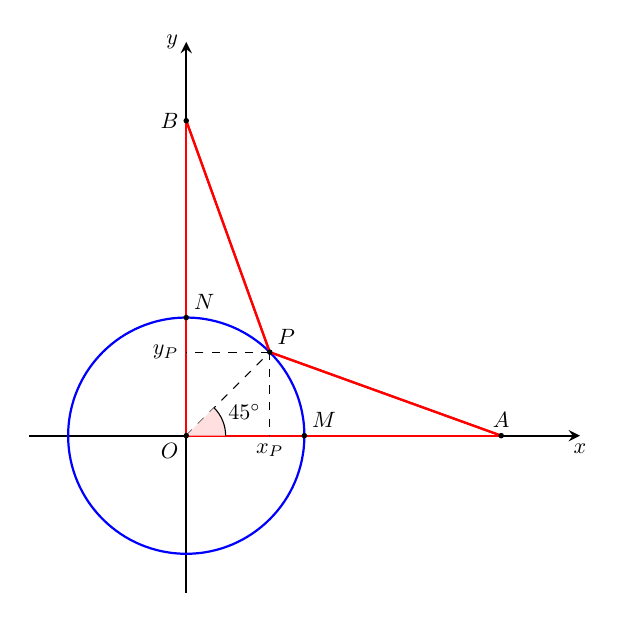
\begin{tikzpicture}[scale=1, >=stealth]
				\tikzset{every node/.style={scale=0.8}}  
				% --- 1. Hệ trục tọa độ ---
				\draw[->, thick] (-2,0) -- (5,0) node[below] {$x$};
				\draw[->, thick] (0,-2) -- (0,5) node[left] {$y$};
				\node[below left] at (0,0) {$O$};
				\coordinate (O) at (0,0);
				\def\R{1.5} % Bán kính
				\draw[thick, blue] (O) circle (\R);
				\coordinate (M) at (\R, 0);
				\coordinate (N) at (0, \R);
				\coordinate (P) at (45:\R);
				\coordinate (A) at (4, 0);
				\coordinate (B) at (0, 4);
				% --- 4. Vẽ các đoạn thẳng (Màu đỏ) ---
				\draw[thick, red] (B) -- (P) -- (A); % Đường gấp khúc BPA
				\draw[thick, red] (B) -- (N); % Đoạn trên trục y (trùng trục nên có thể vẽ đè hoặc offset)
				\draw[thick, red] (A) -- (M); % Đoạn trên trục x
				\draw[thick, red] (B) -- (O) -- (A); % Hai trục
				\draw[thick, red] (B) -- (P) -- (A); % Hai dây cung
				\draw[dashed] (P) -- (P |- O) node[below] {$x_P$};
				\draw[dashed] (P) -- (P -| O) node[left] {$y_P$};
				\draw[dashed] (O) -- (P); % Bán kính OP
				\fill[pink!50] (O) -- (0.5,0) arc (0:45:0.5) -- cycle;
				\draw (0.5,0) arc (0:45:0.5);
				\node at (22.5:0.8) {$45^\circ$};	
				% --- 6. Điểm và Nhãn ---
				\fill (A) circle (1pt) node[above] {$A$};
				\fill (B) circle (1pt) node[left] {$B$};
				\fill (M) circle (1pt) node[above right] {$M$};
				\fill (N) circle (1pt) node[above right] {$N$};
				\fill (P) circle (1pt) node[above right] {$P$};
				\fill (O) circle (1pt);	
			\end{tikzpicture}
		} \noindent
		Tổng quãng đường sẽ ngắn nhất khi con kiến mang miếng mồi thứ $10$ về tổ tại điểm chính giữa cung tròn $MN$ là $P$, và từ đây đến $B$ để lần lượt lấy $3$ miếng mồi còn lại.\\
		Khi đó
		\begin{itemize}
			\item Tổng quãng đường để lấy $10$ miếng mồi ở $A$ là $T_1 = MA\cdot 9\cdot 2 + MA + PA$.
			\item Tổng quãng đường để lấy $3$ miếng mồi ở $B$ là $T_2 = PB + NB + NB\cdot 2\cdot 2$.
		\end{itemize}
		Do đó $T_{\min} = T_1 + T_2 = 19MA + 5NB + PA + PB$.\\
		Ta có
		$\heva{
			&x_P = 6 \cos 45^\circ = 3\sqrt{2} \\
			&y_P = 6 \sin 45^\circ = 3\sqrt{2}
		}\Rightarrow P\left( 3\sqrt{2}; 3\sqrt{2}\right) $.\\
		Suy ra $PA = PB = \sqrt{\left( 20 - 3\sqrt{2}\right)^2 + \left( 3\sqrt{2} - 0\right) ^2} = 2\sqrt{109 - 30\sqrt{2}}$ và $MA = NB = \sqrt{(20 - 6)^2} = 14$.\\
		Vậy $T_{\min} = 19\cdot 14 + 5\cdot 14 + 2\sqrt{109 - 30\sqrt{2}} + 2\sqrt{109 - 30\sqrt{2}} \approx 369$ cm.
	}
\end{ex}

%%%=============BT_5=============%%%
\begin{ex}%[Dự án đề TT THPTQG2026]%[2D1V4-1]
	Đồ thị hàm số $y=\dfrac{x^3\left(\sqrt{x^2-4}+x\right)}{2x^3+3x^2-3x-2}$ có tất cả bao nhiêu đường tiệm cận?
	\par
	%\shortans[0]{3}
	\loigiai{
		Xét $y = \dfrac{x^3\left(\sqrt{x^2-4}+x\right)}{2x^3+3x^2-3x-2}$.\\
		Điều kiện xác định $\heva {&x^2 - 4 \ge 0\\&2x^3+3x^2-3x-2 \ne 0}\Leftrightarrow \heva{&x \in (-\infty; -2] \cup [2; +\infty)\\&x\notin \left\{1;-2;-\dfrac{1}{2}\right\}.}$\\
		Tập xác định $\mathscr {D}=(-\infty; -2) \cup [2; +\infty)$.\\			
		Xét $\lim\limits_{x \to -2^-} \dfrac{x^3\left(\sqrt{x^2-4}+x\right)}{2x^3+3x^2-3x-2}=-\infty$ suy ra $x=-2$ là một đường tiệm cận đứng của đồ thị hàm số.\\		
		Xét $\lim\limits_{x \to -\infty} y = \lim\limits_{x \to -\infty} \dfrac{-4x^3}{(-2x)\left( 2x^3\right) } = \lim\limits_{x \to -\infty} \dfrac{1}{x} = 0$ suy ra $y=0$ là tiệm cận ngang của đồ thị hàm số khi $x \to -\infty$.\\
		Xét $\lim\limits_{x \to +\infty} \dfrac{y}{x} = \lim\limits_{x \to +\infty} \dfrac{x^3\left( \sqrt{x^2-4}+x\right)}{x(2x^3+3x^2-3x-2)} = 1 \Rightarrow a=1$.\\
		Suy ra $\lim\limits_{x \to +\infty} (y-x) = \lim\limits_{x \to +\infty} \left[ \dfrac{x^3\left( \sqrt{x^2-4}+x\right)}{2x^3+3x^2-3x-2} - x\right]   = -\dfrac{3}{2}$.\\
		Vậy $y = x - 1{,}5$ là tiệm cận xiên của đồ thị hàm số khi $x \to +\infty$.\\
		Từ đó ta có 
		\begin{itemize}
			\item Tiệm cận đứng $x = -2$;
			\item Tiệm cận ngang $y = 0$ (khi $x \to -\infty$);
			\item Tiệm cận xiên $y = x - 1{,}5$ (khi $x \to +\infty$).
		\end{itemize} 
		Vậy tổng số đường tiệm cận của đồ thị hàm số đã cho là $3$.
	}
\end{ex}

%%%=============BT_6=============%%%
\begin{ex}%[Dự án đề TT THPTQG2026]%[0D2V2-3]
	Một trang trại dự định dành $100$ ha đất để trồng ba loại cây: cao su, cà phê và hồ tiêu. Lợi nhuận hàng năm ước tính của cao su là $40$ triệu đồng/ha, cà phê là $60$ triệu đồng/ha và hồ tiêu là $80$ triệu đồng/ha. Do các yêu cầu về quy hoạch và nguồn nước, diện tích trồng các loại cây phải tuân thủ các điều kiện sau:
	\begin{enumerate}[1)]
		\item Tổng diện tích trồng cà phê và hồ tiêu không được vượt quá diện tích trồng cao su.
		\item Diện tích trồng hồ tiêu không được vượt quá $20$ ha.
		\item Diện tích trồng cà phê không được vượt quá $3$ lần diện tích trồng hồ tiêu.
	\end{enumerate}
	Tổng lợi nhuận thu được hàng năm của trang trại đó lớn nhất là bao nhiêu tỷ đồng?
	\par
	%\shortans[0]{5,4}
	\loigiai{
		Gọi $x$, $y$, $z$ lần lượt là diện tích đất trồng cao su, cà phê và hồ tiêu (đơn vị: ha).\\
		Điều kiện $x$, $y$, $z \ge 0$.\\
		Tổng diện tích đất là $100$ ha nên ta có phương trình $x + y + z = 100 \Rightarrow x = 100 - (y + z)$.\\
		Các điều kiện ràng buộc khác theo đề bài gồm
		\begin{itemize}
			\item Tổng diện tích trồng cà phê và hồ tiêu không được vượt quá diện tích trồng cao su
			\allowdisplaybreaks
			\begin{eqnarray*}
				y + z \le x &\Leftrightarrow& y + z \le 100 - (y + z)\\ &\Leftrightarrow& 2(y + z) \le 100\\
				& \Leftrightarrow& y + z \le 50.
			\end{eqnarray*}
			\item Diện tích trồng hồ tiêu không được vượt quá $20$ ha suy ra $z \le 20$.
			\item Diện tích trồng cà phê không được vượt quá $3$ lần diện tích trồng hồ tiêu suy ra $y \le 3z$.
		\end{itemize}
		Hàm mục tiêu lợi nhuận (đơn vị: triệu đồng)
		\[L = 40x + 60y + 80z.\]
		Thay $x = 100 - y - z$ vào hàm mục tiêu, ta được
		\[L = 40(100 - y - z) + 60y + 80z = 4000 - 40y - 40z + 60y + 80z = 20y + 40z + 4000.\]
		Bài toán trở thành tìm giá trị lớn nhất của hàm số $F(y, z) = 20y + 40z$ với các điều kiện
		\[\heva{&y \ge 0,\ z \ge 0 \\ &y + z \le 50 \\ &z \le 20 \\ &y \le 3z.}\]	
		Miền nghiệm của hệ bất phương trình là tứ giác $OABC$ như hình vẽ.\\
		Các đỉnh của miền nghiệm tứ giác $OABC$ gồm
		\immini{
			\begin{itemize}
				\item Giao điểm của $y = 0$ và $z = 0$ là gốc tọa độ $O(0; 0)$ suy ra $F = 0$.
				\item Giao điểm của $z = 20$ và $y = 0$ là điểm $C(20; 0)$ suy ra $F = 20\cdot 0 + 40\cdot 20= 800$.
				\item Giao điểm của $z = 20$ và $y + z = 50$ là điểm $B$ có tọa độ thỏa
				$$\heva{&z = 20 \\ &y + 20 = 50} \Leftrightarrow \heva{&z = 20 \\ &y = 30.}$$
				Vậy $B(20; 30)$ suy ra $$F = 20\cdot 30+ 40\cdot 20 = 600 + 800 = 1\,400.$$
				\item Giao điểm của $y = 3z$ và $y + z = 50$ là điểm $A$ có tọa độ thỏa
				$$\heva{&y = 3z \\ &3z + z = 50}\Leftrightarrow \heva{&z = 12{,}5 \\ &y = 37{,}5.}$$
				Vậy $A( 12{,}5;37{,}5)$ suy ra $$F = 20\cdot 37{,}5 + 40\cdot 12{,}5 = 750 + 500 = 1\,250.$$
			\end{itemize}
		}{
			\begin{tikzpicture}[scale=0.12,line join=round, line cap=round,>=stealth]			
				% --- 1. Thiết lập hệ trục tọa độ ---
				\draw[->] (-5,0) -- (60,0) node[above] {$z$ (hồ tiêu)};
				\draw[->] (0,-5) -- (0,60) node[right] {$y$ (cà phê)};
				\node[below left] at (0,0) {$O$};				
				% --- 2. Vẽ các đường thẳng giới hạn ---	
				% Đường y + z = 50 => y = 50 - z
				\draw[thick, name path=line1] (-5, 55) -- (55, -5) node[pos=0.7, sloped,above] {$y+z=50$};	
				% Đường z = 20 (Thẳng đứng)
				\draw[thick, name path=line2] (20, 0) -- (20, 60) node[pos=0.8,sloped,below] {$z=20$};	
				% Đường y = 3z
				\draw[thick, name path=line3] (0, 0) -- (18, 54) node[pos=0.9, sloped,above] {$y=3z$};	
				% --- 3. Xác định các đỉnh của miền nghiệm ---
				\coordinate (A) at (12.5, 37.5);	
				\coordinate (B) at (20, 30);	
				\coordinate (O) at (0,0);
				\coordinate (C) at (20,0);	
				% --- 4. Tô màu miền nghiệm ---
				\fill[pattern=north east lines, pattern color=green!50!black, opacity=0.5] (O) -- (A) -- (B) -- (C) -- cycle;
				\draw[ultra thick, green!40!black] (O) -- (A) -- (B) -- (C) -- cycle;	
				% --- 5. Đánh dấu các đỉnh ---
				\fill (O) circle (12pt) node[below left] {$O$};
				\fill (A) circle (12pt) node[right] {$A$};
				\fill (B) circle (12pt) node[right] {$B$};
				\fill (C) circle (12pt) node[above right] {$C$};					
				% Các đường gióng (Tùy chọn)
				\draw[dashed] (12.5, 0) node[below] {$12{,}5$} -- (A) -- (0, 37.5) node[left] {$37{,}5$};
				\draw[dashed] (20, 0) node[below] {$20$} -- (B) -- (0, 30) node[left] {$30$};	
			\end{tikzpicture}
		}\noindent
		So sánh các giá trị $F$, ta thấy giá trị lớn nhất là $F_{\max} = 1\,400$ tại điểm $B(20; 30)$.\\
		Khi đó, lợi nhuận lớn nhất của trang trại là
		\[L_{\max} = 1\,400 + 4\,000 = 5\,400 \text{ (triệu đồng)}= 5{,}4 \text{ (tỷ đồng)}.\]	
	}
\end{ex}



\Closesolutionfile{ans}

%\indapan{6}{ans/ans-26-2--SoGD-L1-LC}
%\indapan{4}{ans/ans-26-2--SoGD-L1-DS}
%\indapan{6}{ans/ans-26-2--SoGD-L1-KQ}
